\documentclass[a4paper,10pt]{article}

%A Few Useful Packages
\usepackage{marvosym}
\usepackage{fontspec} 					%for loading fonts
\usepackage{xunicode,xltxtra,url,parskip} 	%other packages for formatting
\RequirePackage{color,graphicx}
\usepackage[usenames,dvipsnames]{xcolor}
\usepackage[big]{layaureo} 				%better formatting of the A4 page
% an alternative to Layaureo can be ** \usepackage{fullpage} **
\usepackage{supertabular} 				%for Grades
\usepackage{titlesec}					%custom \section
\usepackage{tabu}
\usepackage{multirow}
\usepackage{hyperref}

%Setup hyperref package, and colours for links
\usepackage{hyperref}
\definecolor{linkcolour}{rgb}{0,0.2,0.6}
\hypersetup{colorlinks,breaklinks,urlcolor=linkcolour, linkcolor=linkcolour}

%FONTS
\defaultfontfeatures{Mapping=tex-text}
%\setmainfont[SmallCapsFont = Fontin SmallCaps]{Fontin}
%%% modified for Karol Kozioł for ShareLaTeX use
\setmainfont[
SmallCapsFont = Fontin-SmallCaps.otf,
BoldFont = Fontin-Bold.otf,
ItalicFont = Fontin-Italic.otf
]
{Fontin.otf}
%%%

%CV Sections inspired by: 
%http://stefano.italians.nl/archives/26
\titleformat{\section}{\Large\scshape\raggedright}{}{0em}{}[\titlerule]
\titlespacing{\section}{0pt}{3pt}{3pt}
%Tweak a bit the top margin
%\addtolength{\voffset}{-1.3cm}

%Italian hyphenation for the word: ''corporations''
\hyphenation{im-pre-se}

%-------------WATERMARK TEST [**not part of a CV**]---------------
\usepackage[absolute]{textpos}

\setlength{\TPHorizModule}{30mm}
\setlength{\TPVertModule}{\TPHorizModule}
\textblockorigin{2mm}{0.65\paperheight}
\setlength{\parindent}{0pt}

%--------------------BEGIN DOCUMENT----------------------
\begin{document}

\pagestyle{empty} % non-numbered pages

\font\fb=''[cmr10]'' %for use with \LaTeX command

%--------------------TITLE-------------


  \begin{tabular}{ p{11cm}r }
   %& %\multirow{1}{2in}%{
   %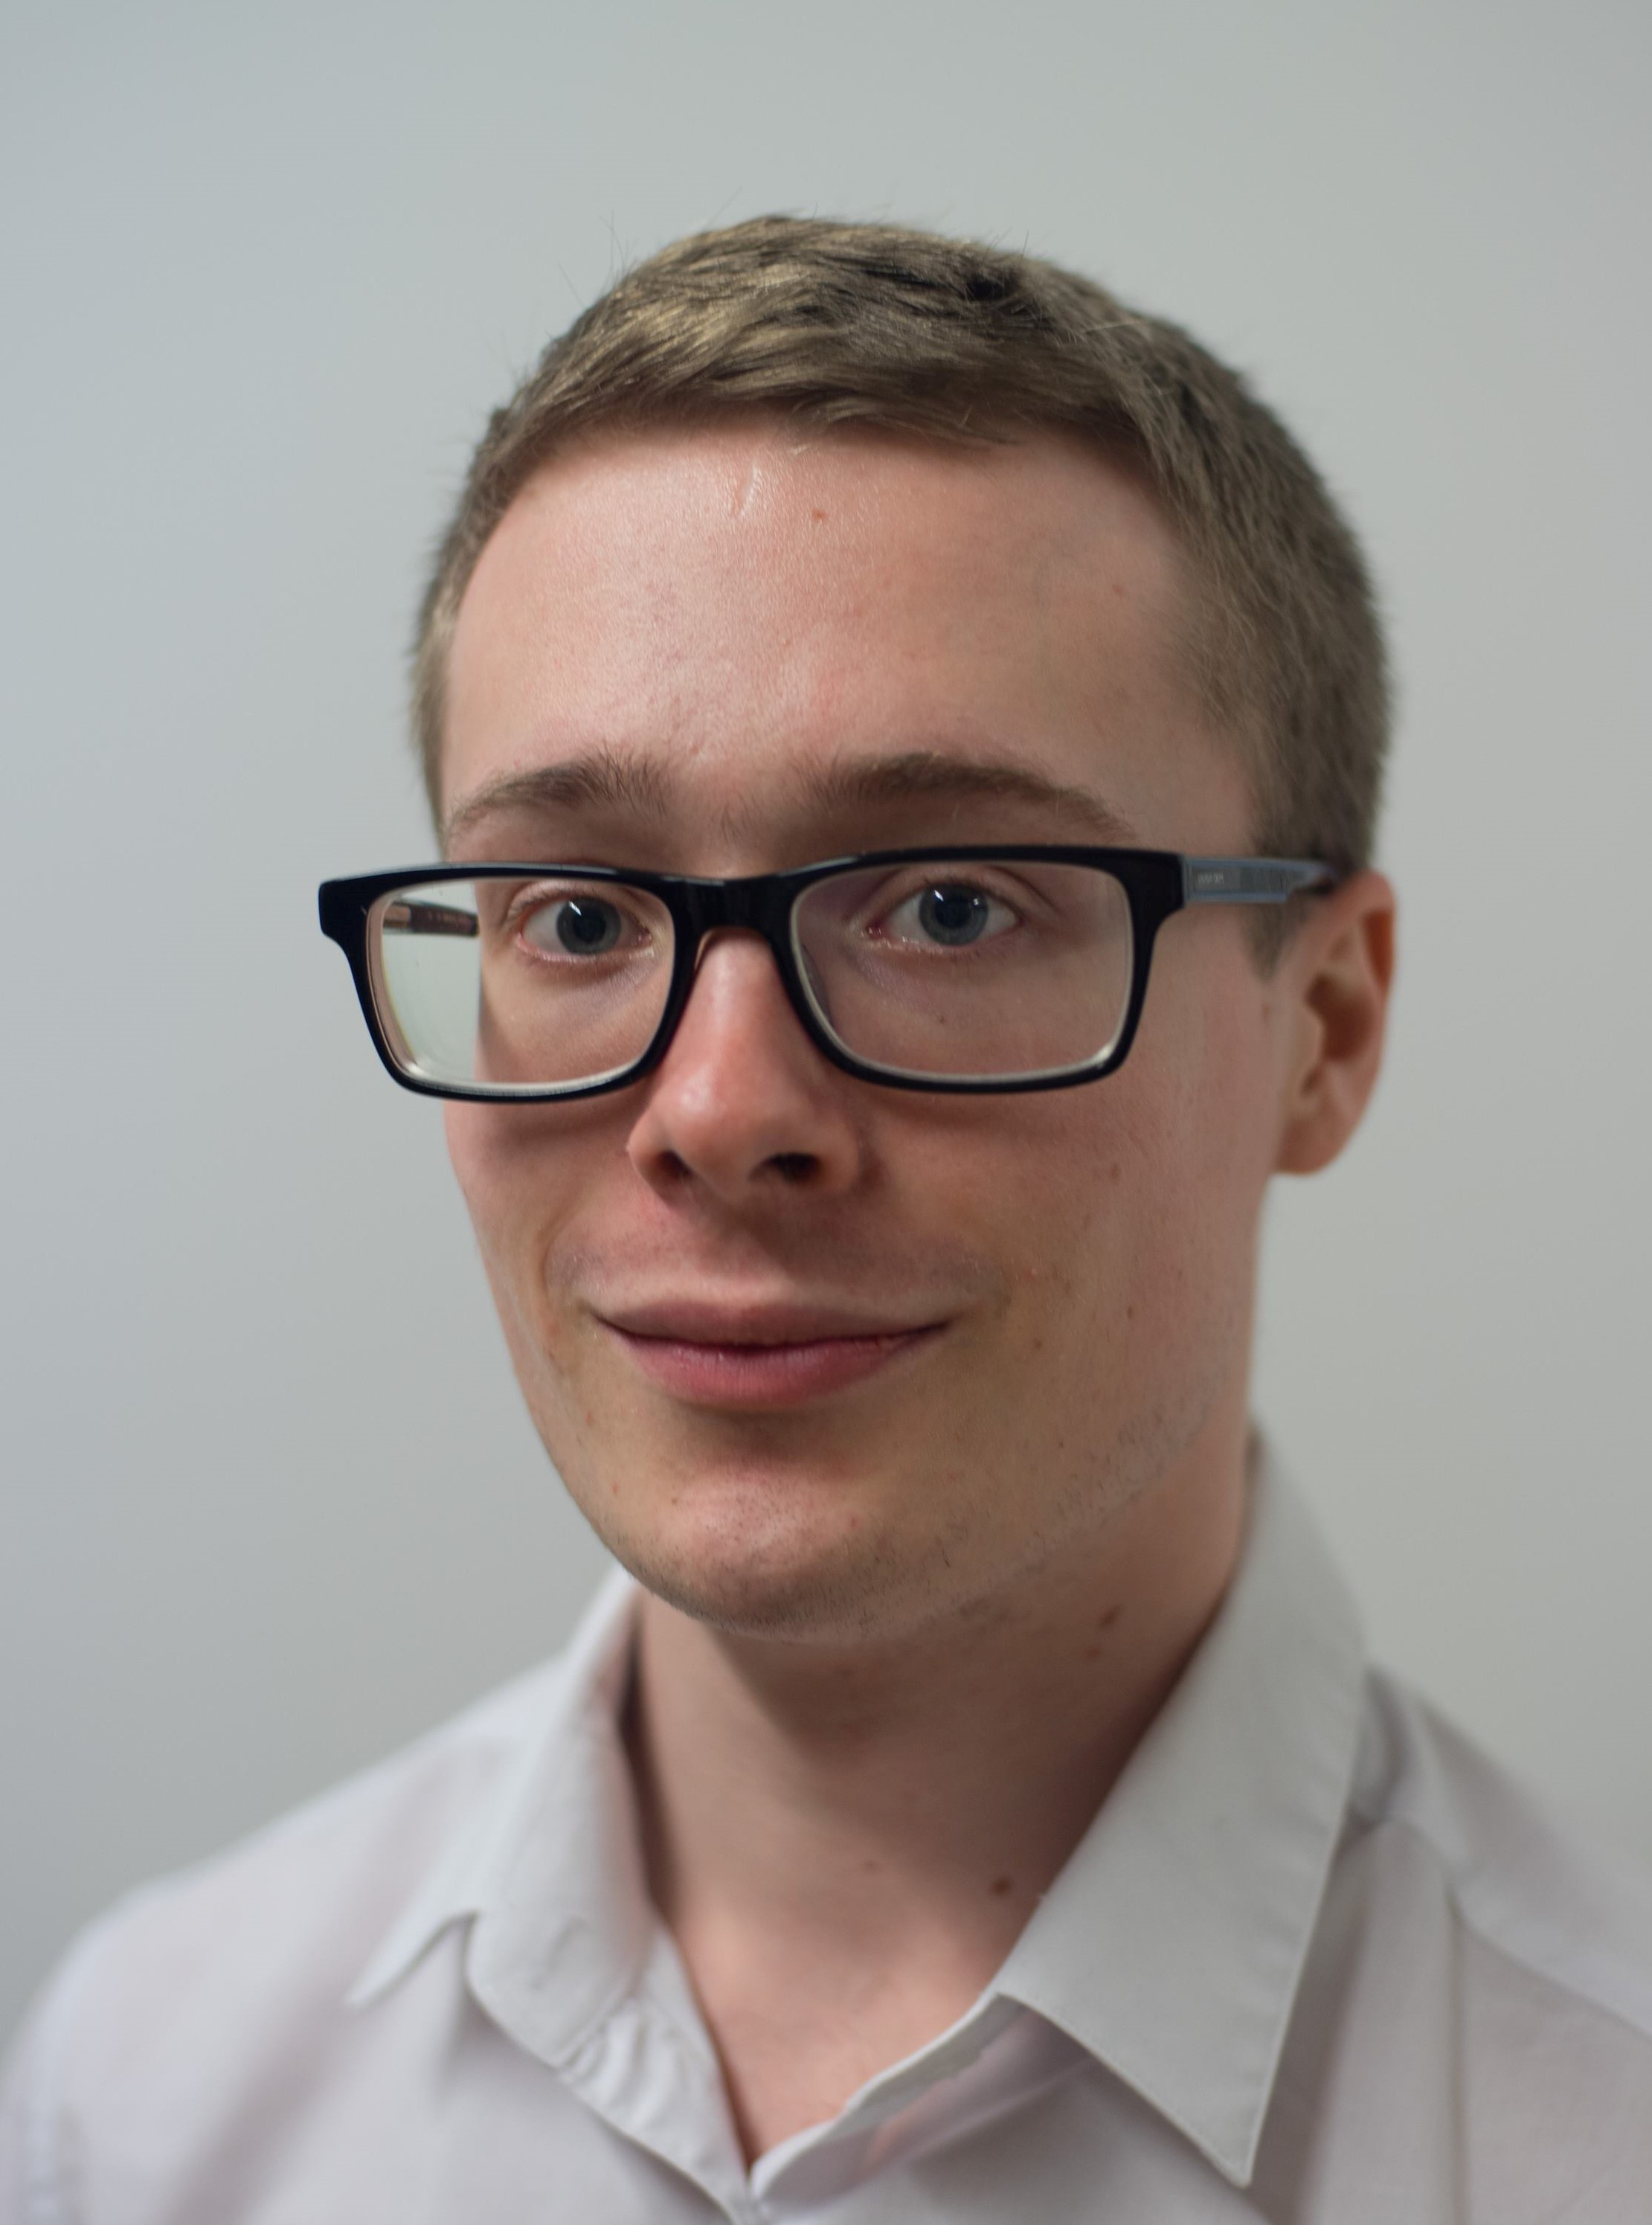
\includegraphics[width=1.5in]{pic}\\
   %} \\
   & \multirow{5}{2in}{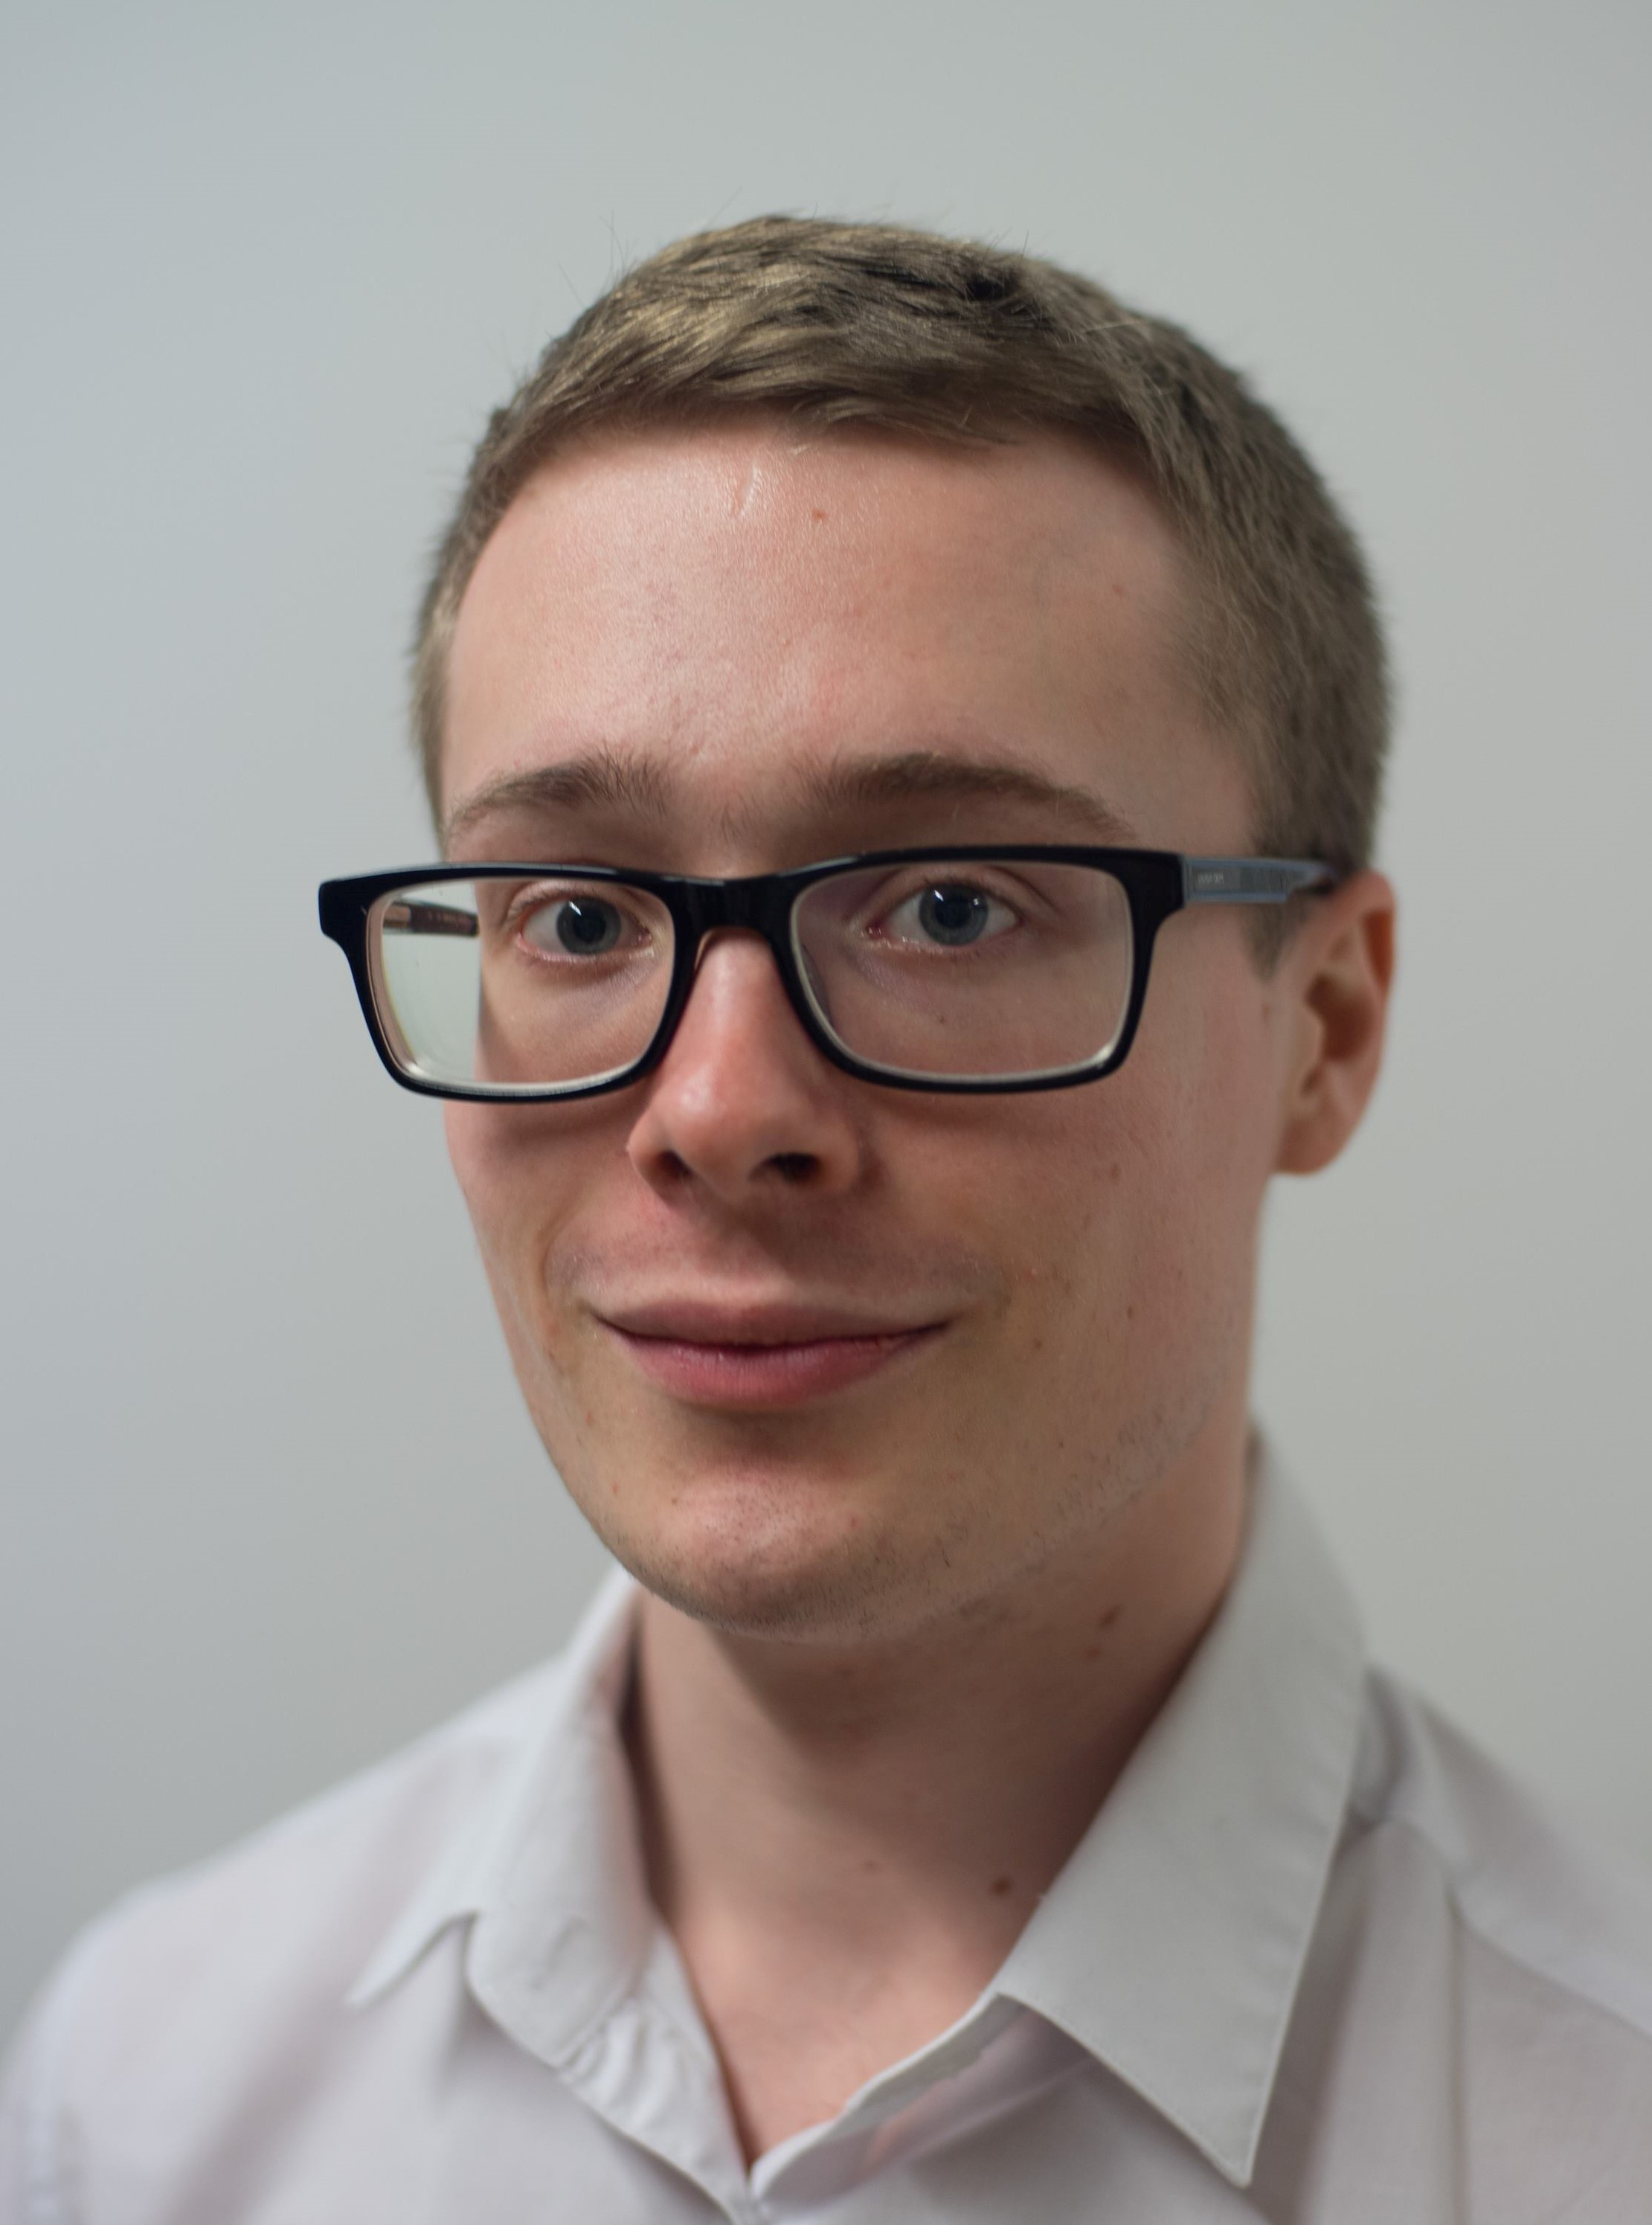
\includegraphics[width=1.5in]{pic}}\\
   \scshape{\Huge{Charles Nourry}} & \\
   \\
   \textsc{Age:} 21 ans &\\
    \textsc{Address:} 1 rue de la ferme &\\
    \textsc{Ville:} 78150 - Le Chesnay&\\
    \textsc{Phone:} 06 21 09 85 62&\\
    \textsc{email:} \href{mailto:nourry\_charles@outlook.fr}{nourry\_charles@outlook.fr}& %\multirow{5}{2in}{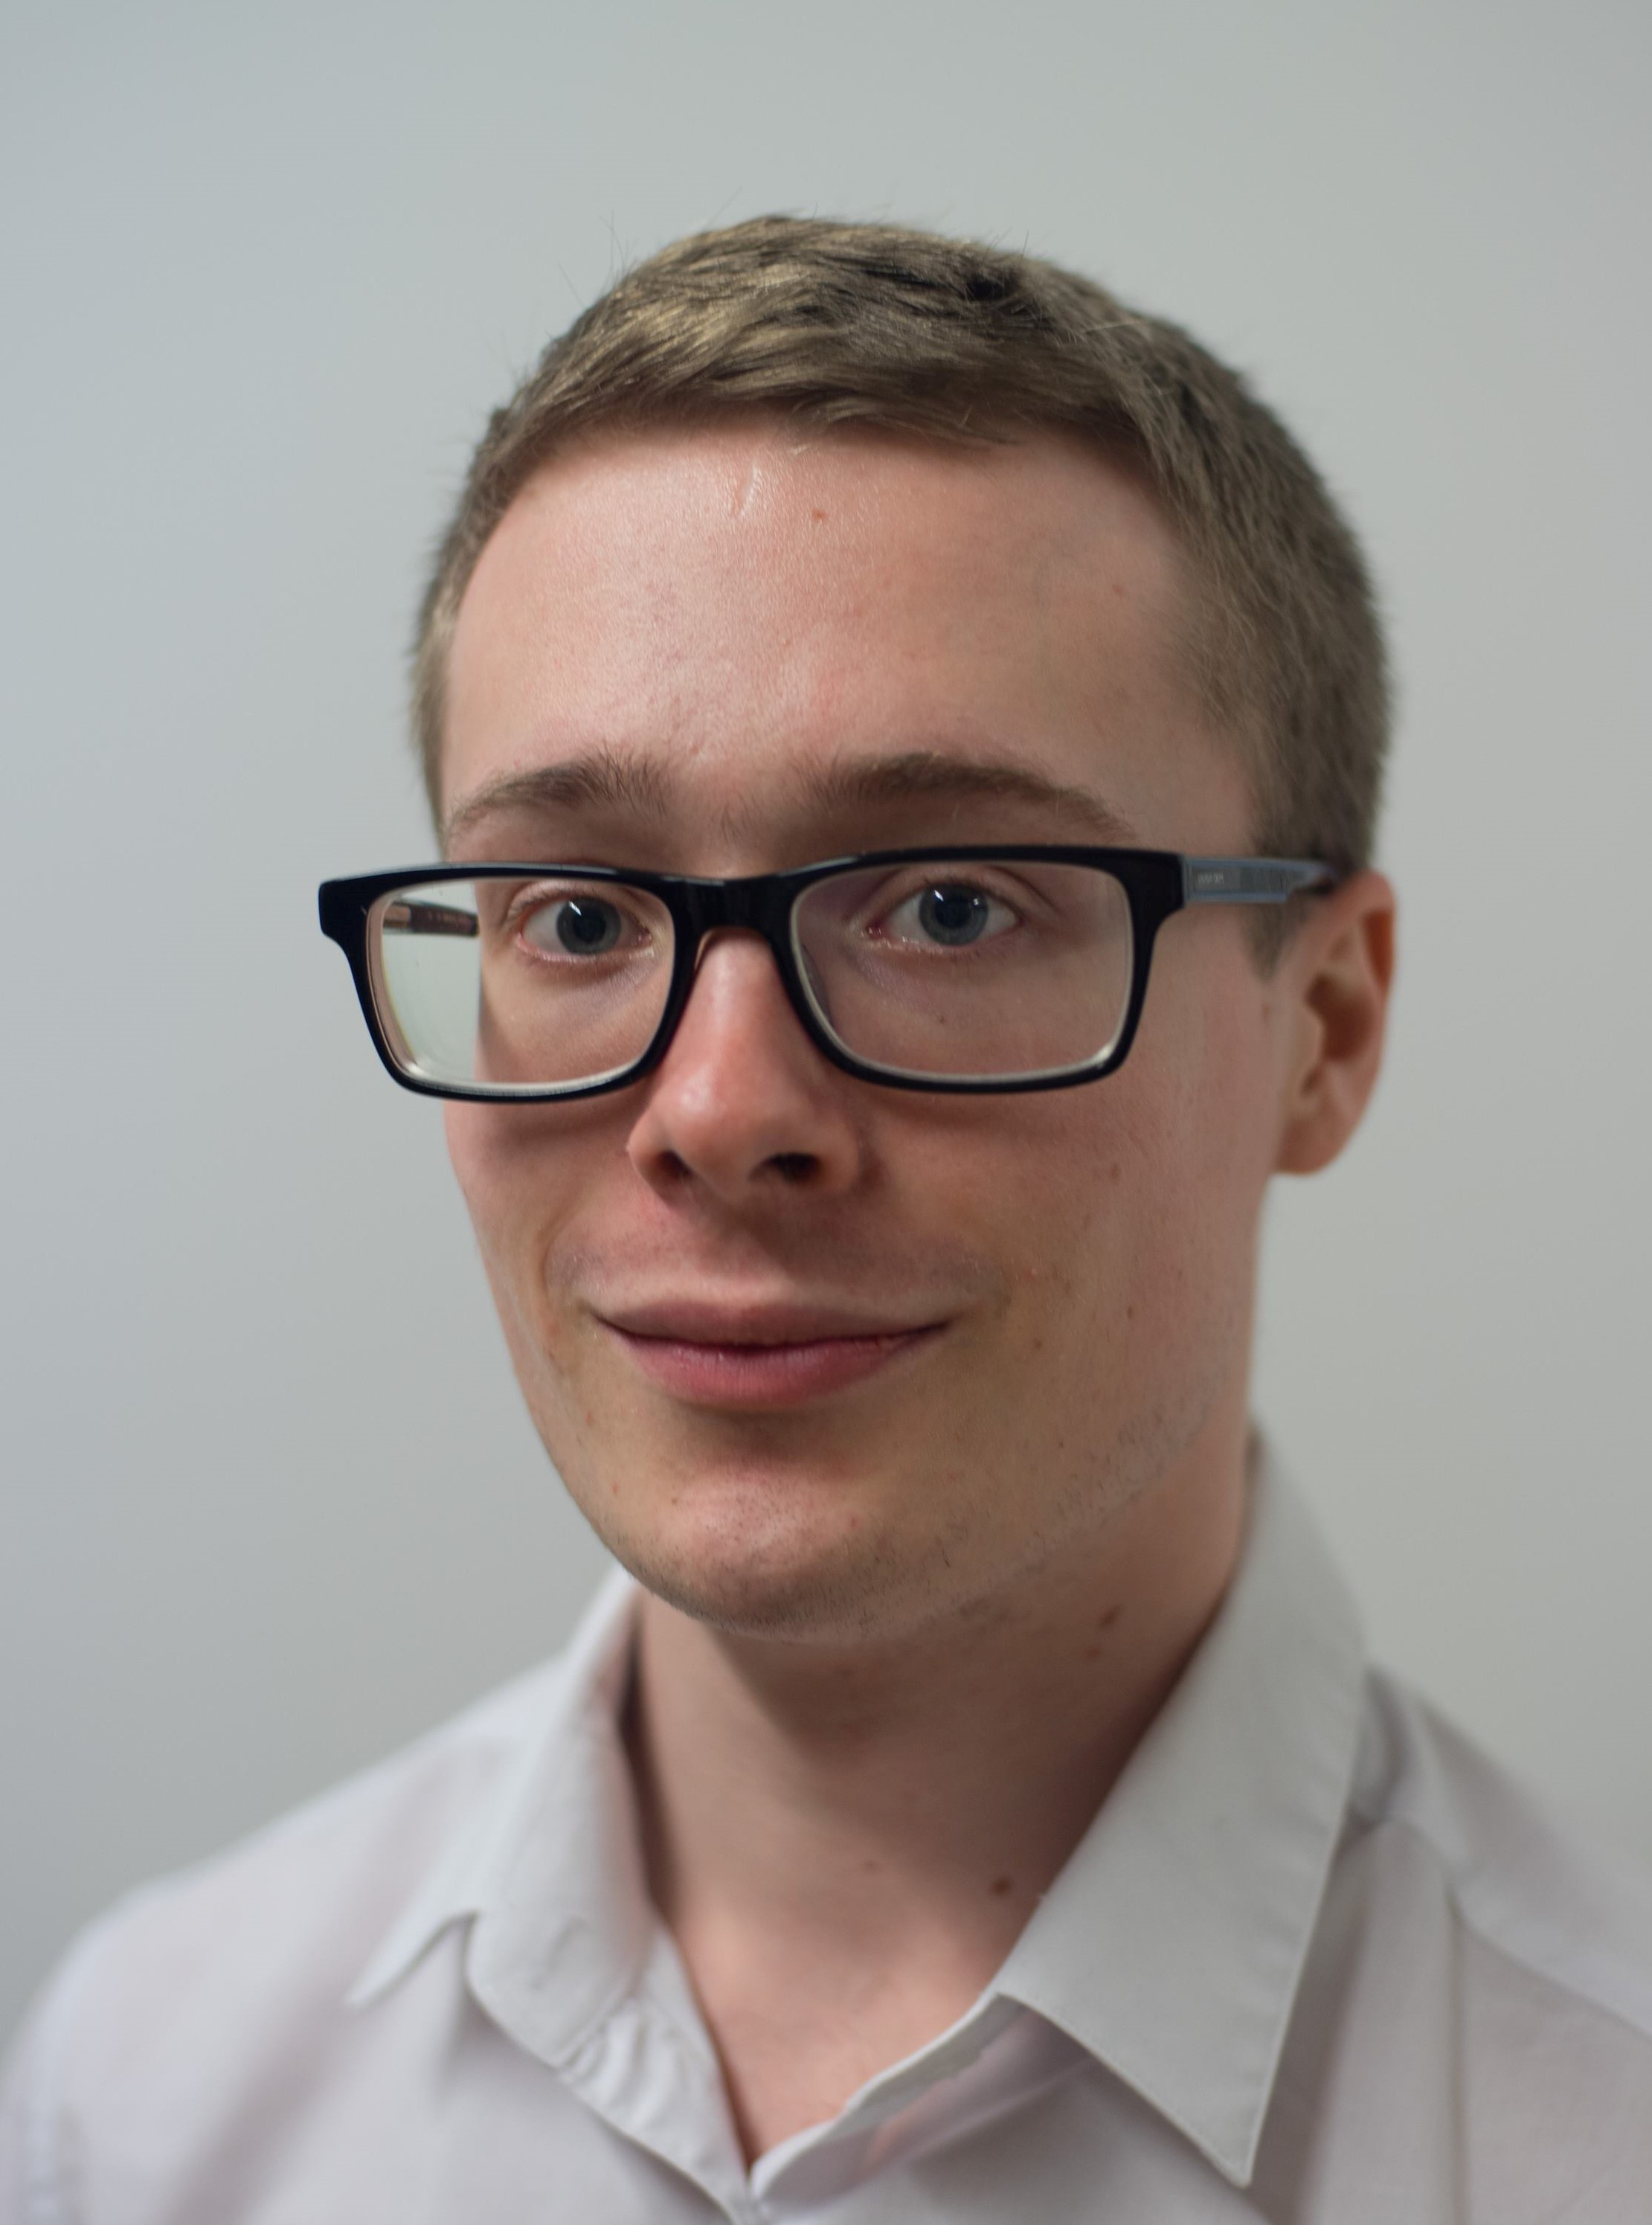
\includegraphics[width=1.5in]{pic}}
  \end{tabular}

%\par{%\centering{
%	\Large
%	Charles \textsc{Nourry}
	%}
%	\bigskip\par}
%\normalsize
%--------------------SECTIONS-----------------------------------
%Section: Personal Data
%\section{Personal Data}

%\begin{tabular}{ll}
 %   \textsc{Age:} & 20 \\
  %  \textsc{Address:}   & 1 rue de la ferme \\
%    \textsc{Ville:} 	& 78150 - Le Chesnay\\
 %   \textsc{Phone:}     & 06 21 09 85 62\\
  %  \textsc{email:}     & $\href{mailto:nourry_charles@outlook.fr}{nourry_charles@outlook.fr}$
%\end{tabular}

%Section: Work Experience at the top
\section{Formation}
\begin{tabular}{r|p{11cm}}
 \textsc{2017-2019} & Master MODO \\&\emph{\small{Université Paris-Dauphine, Paris}}\\\multicolumn{2}{c}{} \\
 \textsc{2016-2017} & Licence Informatique des organisations - MIAGE et Décision \\&\emph{\small{Université Paris-Dauphine, Paris}}\\\multicolumn{2}{c}{} \\
 \textsc{2014-2016} & Diplôme d'Etablissement Mathématiques, Informatique et applications à l'Economie et à l'Entreprise (L1 \& L2) \\&\emph{\small{Université Paris-Dauphine, Paris}}\\\multicolumn{2}{c}{} \\
 \textsc{2014} & Baccalauréat Scientifique option Mathématiques \\&\emph{\small{Lycée Blanche de Castille, Le Chesnay}}\\
\end{tabular}

\section{Compétences}
\begin{tabular}{rl}	
 Développement & Programmation orientée objet, Java, C, Python, R, Matlab, \LaTeX, VBA\\&\\
Système d'exploitation & Microsoft Windows, Linux\\&\\
Logiciels & Word, Excel, PowerPoint, Access, Eclipse, IntelliJ, LaTeX, Jupyter Notebook, RStudio, MySQL
\end{tabular}

\section{Expériences personnelles}
\begin{tabular}{rl}	
 \textsc{Mai} 2017 - \textsc{Août} 2017 & Stage de Licence au \textsc{Crédit Industriel et Commercial}\\&
 \emph{\small{Mise en place d'outils informatique}}\\&\\
 \textsc{Mai} 2018 - \textsc{Août} 2018 & Stage de recherche au \textsc{LAMSADE} Labo... Université Paris-Dauphine\\&
 \emph{\small{Analyse de débats en ligne, théorie de l'argumentation}}\\&\\
 \textsc{Mai} 2017 - \textsc{Août} 2017 & Projets
\end{tabular}

%Section: Languages
\section{Langues}
\begin{tabular}{rl}
\textsc{Français:}&Langue maternelle\\
\textsc{Anglais:}&compétence professionnelle\\
\textsc{Espagnol:}&Occasionnelle\\
\end{tabular}

\section{Centres d'intérêt}
Piano, Cinéma, Athlétisme


%Section: Education
\section{Education}
\begin{tabular}{rl}	
 \textsc{July} 2008 & Master of Science in \textsc{Finance}, \textbf{Bocconi University}, Milan\\
& 110/110 \small\emph{summa cum laude} | Major: Quantitative Finance\\
& Thesis: ``Sublinear and Locally Sublinear Prices'' | \small Advisor: Prof. Erio \textsc{Castagnoli}\\
&\normalsize \textsc{Gpa}: 28.61/30\hyperlink{grds}{\hfill | \footnotesize Detailed List of Exams}\\&\\
\textsc{July} 2006& Undergraduate Degree in \textsc{Law} and \textsc{Business Administration} \\&110/110 \small\emph{summa cum laude}, \normalsize\textbf{Bocconi University}, Milan\\
& Thesis: ``Portfolio Strategies with Target Prices'' | \small Advisor: Stefano \textsc{Bonini}\\
&\normalsize \textsc{Gpa}: 29.85/30\hyperlink{grds_cleli}{\hfill| \footnotesize Detailed List of Exams}\\&\\
\textsc{Fall} 2005& Exchange Semester at \textbf{University of Southern California}, Los Angeles\\
&\textsc{Gpa}: 3.875/4 \hyperlink{grds_usc}{\hfill| \footnotesize Detailed List of Exams}\\&\\
\textsc{July} 2003& \textbf{Liceo Classico ``E. Duni''}, Matera | Final Grade: 100/100
\end{tabular}

%Section: Scholarships and additional info
\section{Scholarships and Certificates}
\begin{tabular}{rl}
 \textsc{Sept.} 2006 & Scholarship for graduate students with an outstanding curriculum \footnotesize(\EURcr 30,000)\normalsize\\
\textsc{June} 2006 & {\textsc{Gmat}\textregistered}\setmainfont[SmallCapsFont=Fontin-SmallCaps.otf]{Fontin.otf}: 730 (\textsc{q:50;v:39}) 96\textsuperscript{th} percentile; \textsc{awa}: 6.0/6.0 (89\textsuperscript{th} percentile)
\end{tabular}

%Section: Languages
\section{Languages}
\begin{tabular}{rl}
 \textsc{Italian:}&Mothertongue\\
\textsc{English:}&Fluent\\
\textsc{French:}&Basic Knowledge\\
\end{tabular}

\section{Computer Skills}
\begin{tabular}{rl}
 Basic Knowledge:& \textsc{php}, my\textsc{sql}, \textsc{html}, Access, \textsc{Linux}, ubuntu, {\fb \LaTeX}\setmainfont[SmallCapsFont=Fontin-SmallCaps.otf]{Fontin.otf}\\
Intermediate Knowledge:& \textsc{vba}, Excel, Word, PowerPoint\\
\end{tabular}

\section{Interests and Activities}
Technology, Open-Source, Programming\\
Paradoxes in Decision Making, Psychoanalysis, Behavioural Finance\\
Football, Travelling


%\XeTeXpdffile ''GMAT.pdf'' page 1 scaled 800

\end{document}
